\documentclass[a4paper,12pt]{article} % тип документа

% report, book

%  Русский язык
\usepackage{multirow}
\usepackage{wrapfig}
\usepackage[T2A]{fontenc}			% кодировка
\usepackage[utf8]{inputenc}			% кодировка исходного текста
\usepackage[english,russian]{babel}	% локализация и переносы

\usepackage{indentfirst} %Красная строка
\usepackage[a4paper,top=1.3cm,bottom=2cm,left=1.5cm,right=1.5cm,marginparwidth=0.75cm]{geometry}
\usepackage[usenames]{color}
\usepackage{colortbl}

% Заметки
\usepackage{todonotes}

% Математика
\usepackage{amsmath,amsfonts,amssymb,amsthm,mathtools} 
\usepackage{hyperref}

\begin{document}

\begin{titlepage}
\begin{center}
    {\large МОСКОВСКИЙ ФИЗИКО-ТЕХНИЧЕСКИЙ ИНСТИТУТ (НАЦИОНАЛЬНЫЙ ИССЛЕДОВАТЕЛЬСКИЙ УНИВЕРСИТЕТ)}
\end{center}
\begin{center}
    {\largeФизтех-школа биологической и медицинской физики}
\end{center}


    \vspace{3.5cm}

\begin{center}
    
\includegraphics[width=0.4\linewidth]{hv_full.png}
\end{center}
\vspace{0.1cm}
{\huge
\begin{center}
    {\bf Лабораторная работа 7.4A}\\
    Исследование поглощения вторичного космического излучения в свинце
\end{center}
}
\vspace{2cm}
\begin{flushright}
{\LARGE Авторы:\\ Ирина Веретененко \\
\vspace{0.2cm}
Б06-804}
\end{flushright}
\vspace{3.5cm}
\begin{center}
    Долгопрудный 2020
\end{center}
\end{titlepage}

\newpage

\section{Введение}

\textbf{Цель работы}:
\begin{itemize}
    \item Изученить зависимость интенсивности падающего космического излучения на уровне моря от толщины пройденных им свинцовых пластин 
    \item Найти отношение интенсивностей мягкой и жесткой компонент космического излучения.
\end{itemize}
 

\textbf{В работе используются}: 
\begin{itemize}
    \item космический телескоп с двумя детекторами (счетчиками Гейгера-Мюллера), регистрирующий количество прошедших через оба детектора частиц
    \item блок управления и индикации (БУИ)
    \item блоки из свинца
\end{itemize}


\subsection{Теория}

\subsubsection{Космическое излучение}
\textbf{Космические лучи }- поток частиц высокой энергии (до $10^{20}$эВ), преимущественно протонов, приходящих на Землю из мирового пространства (\textbf{первичное излучение}), а также рожденное ими в атмосфере Земли в результате взаимодействия с атомными ядрами воздуха  \textbf{вторичное излучение}, в котором встречаются практически все элементарные частицы. \\\\
\begin{figure}[h!]
\center{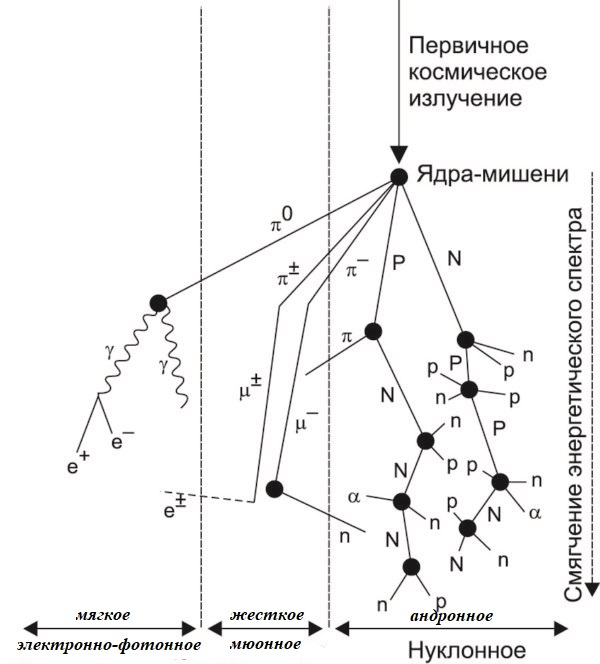
\includegraphics[scale=2]{схема излучения.jpg}}
\caption{Схема превращений первичного космического излучения в атмосфере}
\label{схема}
\end{figure}
На рис \ref{схема} преставлено схематичное изображение взаимодействия первичного протона с атмосферой Земли. Можно увидеть, что образованное при таком взаимодействии вторичное излучение имеет три компоненты:
\begin{itemize}
    \item \textbf{ядерно-активная(андронная)}  $\pi, p, n$
    \item \textbf{жесткая (мюонная)}  $\pi^{+} \rightarrow \mu^{+} + \nu_{\mu}, \pi^- \rightarrow \mu_- +  \widetilde{\nu_{\mu}}$, где $\nu_\mu$ и $\widetilde{\nu_{\mu}}$ - мюонные нейтрино и антинейтрино
    \item \textbf{мягкая (электронно-фотонная)} $\pi^0 \rightarrow \gamma + \gamma$
\end{itemize}
В данной работе исследуется поглощение свинцом вторичного космического излучения на уровне моря. До этого уровня доходят 2 компоненты космического излучения: жесткая и мягкая. Остановимся на каждой из них подробнее.

\subsubsection{Мягкая компонента}
Мягкая компонента состоит из электронов, позитронов и $\gamma$-квантов (фотонов с высокой энергией). \\
\begin{figure}[h!]
\center{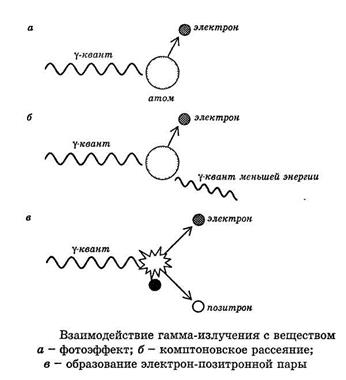
\includegraphics[scale=1]{взаимодействия гамма квантов с веществом.jpg}}
\caption{Основные механизмы взаимодействия $\gamma$-кванта с атомом}
\label{мягкая}
\end{figure}
Существует 3 основных механизма взаимодействия $\gamma$-квантов с атомом (см. \ref{мягкая}):
\begin{itemize}
    \item\textbf{ Фотоэффект} - $\gamma$-квант целиком поглощается атомом, при этом один из электронов атомной оболочки "выбивается" из атома. 
    \item \textbf{Эффект Комптона} - рассеяние $\gamma$-квантов на свободном электроне (энергия связи которого много меньше энергии первичного $\gamma$-кванта). При эффекте Комптона в конечном состоянии наблюдается электрон и вторичный фотон с более низкой энергией.
\end{itemize}
Данные эффекты происходят при достаточно низких энергиях фотонов, поэтому в атмосфере (где фотоны высокоэнергичные) они не наблюдаются. 
\begin{itemize}
    \item  \textbf{Эффект образования электронно-позитронной пары} $\gamma \rightarrow e^+ + e^-$. Важно отметить, что такой распад не может произойти без участия атомов, так как это привело бы к нарушению ЗСЭ и ЗСИ. Данный процесс происходит в кулоновском поле частицы, которая забирает часть энергии и импульса. Поэтому этот механизм реализуется для высокоэнергетичных $\gamma$-квантов $E_\gamma \geqslant
2m_ec^2 + E \sim 2\cdot 0.511\text{МэВ} + 5 \text{КэВ} \sim 1.022\text{МэВ}$, где E - энергия отдачи ядра.\\\\
В атмосфере появившиеся электроны и позитроны испускают тормозные $\gamma$-кванты. Это происходит из-за того, что они движутся в электростатических полях атомных ядер и электронов. Такое излучение называется \textbf{тормозным}. Стоит отметить, что интенсивность тормозного излучения $I \sim a^2 \sim \frac{1}{m}$, поэтому оно вносит больший вклад для частиц с меньшей массой. \\\\
Полученные $\gamma$-кванты снова рождают электроны и позитроны. Такой лавинообразный процесс в атмосфере идет до тех пор, пока ионизационные потери электронов и позитронов (потери, идущие на ионизацию атомов) не сравняются с их радиационными потерями (потери на излучение). Это происходит в воздухе при энергиях порядка 70 МэВ
\\
Можно показать, что (Z-заряд ядра атома)
\begin{equation*}
    \sigma_{\text{пар}}\sim Z^2
\end{equation*}
Rem: Эффективное сечение характеризует вероятность протекания той или иной реакции ($\Phi$ - поток фотонов [$\frac{\text{частицы}}{\text{см}^2}$], $\frac{\Delta N}{N}$ - вероятность распада (отношение числа прореагировавших частиц ко исходному числу частиц). 
$\frac{\Delta N}{N} = \sigma \Phi$)
Видно, что сечение имеет размерность площади. 

\end{itemize}

\textit{
В итоге, от мягкого рентгеновского излучения на поглощающее вещество падают $\gamma$-кванты с высокими энергиями. Они поглощаются веществом за счет образования электронно-позитронных пар, испускающих новые кванты за счет тормозного излучения. Энергия новых квантов меньше, так как электроны и позитроны отдают им только часть своей энергии. Процесс идет до тех пор, пока энергия очередного $\gamma$-кванта не станет меньше пороговой для образования пары. Тогда излучение поглотится полностью}\\
Выведем зависимость интенсивности мягкого излучения от толщины поглощающего слоя:\\
Рассмотрим слой вещества толщины $dx$. В нем $nSdx$ атомов поглощающего вещества (n - концентрация атомов). Тогда уменьшение интенсивности излучения в слое $dI = -\sigma_{\text{пар}}n dx \Rightarrow \boxed{I_{\text{м}} = I_{\text{м}_0} e^{-\sigma_{\text{пар}}nx}, \sigma_{\text{пар}} \sim Z^2} $

\subsubsection{Жесткая компонента}
Жесткая компонента состоит из $\mu$-мезонов, которые слабо поглощаются веществом, притом приблизительно одинаково веществами с разными Z. Это происходит из-за того, что мюоны практически не теряют энергию за счет тормозного излучения (их масса сильно больше массы электронов, поэтому интенсивность тормозного излучения мюонов сильно меньше). Потери энергии мюонов происходят только за счет ионизации атомов, и эти потери практически постоянны, не зависят от состава вещества. Поэтому $\boxed{I_{\text{ж}} = I_{\text{ж}_0}}$ 

\subsubsection{Ожидаемые результаты}
В данной работе будет измерена интенсивность I прошедшего через вещество толщины x вторичного космического излучения. Из предыдущих пунктов:
\begin{equation} \label{!!!}
    \boxed{I(x) = I_{\text{ж}} + I_{\text{м}} = I_{\text{ж}_0} + I_{\text{м}_0} e^{-\sigma_{\text{пар}}nx}}
\end{equation}


\subsection{Экспериментальная установка}
\begin{figure}[h!]
\center{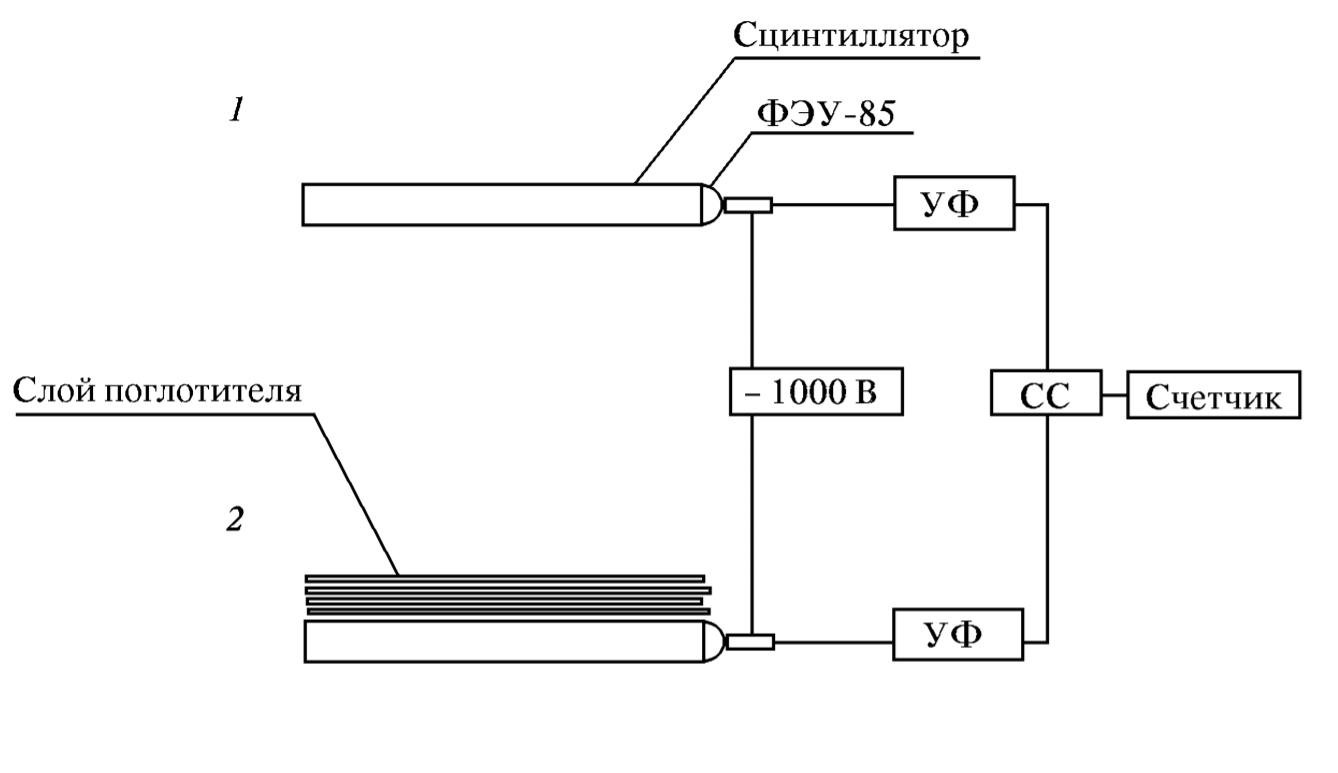
\includegraphics[scale=0.3]{установка.png}}
\caption{Теоретический вид экспериментальной установки}
\label{fig:image1}
\end{figure}
\begin{figure}[h!]
\center{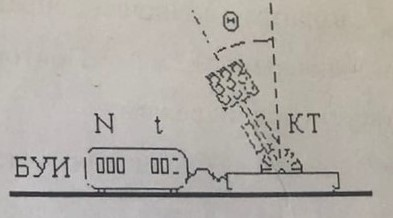
\includegraphics[scale=0.5]{установка_1.png}}
\caption{Экспериментальная установка}
\label{fig:image2}
\end{figure}
\begin{itemize}
    \item 

Основа установки(\ref{fig:image1})(\ref{fig:image2}) - космический телескоп КТ, регистрирующий частицы, приходящие на детекторы в определенном направлении внутри телесного угла.
 Космические частицы регистрируются счетчиками Гейгера-Мюллера 1
и 2; если частица пройдет через оба детектора
то схема совпадений вырабатывает импульс. Если частица
проходит через один из детекторов и не попадает во второй
детектор, тогда схема совпадений импульс не
вырабатывает. Таким образом, число импульсов, сосчитанных пересчетным прибором, должно быть равным числу частиц, прошедших через оба детектора и зарегистрированных ими.
В отсутствии поглощающих фильтров между детекторами установка будет регистрировать частицы как жесткой, так и мягкой компоненты космического излучения.
Если же между детекторами поместить поглотитель (свинец), то частицы мягкой компоненты будет поглощаться в поглотителе. Это приведет к заметному уменьшению скорости счета совпадений.\\
\item
Блок управления и индикации (БУИ) установки содержит:
\begin{itemize}
    \item таймер с максимальным временем измерения 999 с;
    \item высоковольтный выпрямитель для питания счетчиков;
    \item схему совпадений;
    \item блок пересчета импульсов.
\end{itemize}
\item
В БУИ имеются следующие кнопки управления:
\begin{itemize}
    \item Сеть (на задней панели прибора) - включает питание блоков 220 В.
    \item Пуск - включает таймер и отсчет измеряемых импульсов одновременно
    \item Стоп - одновременная их остановка.
    \item Сброс - обнуляет их показания.
    \item Время - устанавливает необходимое время измерения.
\end{itemize}

\end{itemize}
\newpage
\section{Ход работы и обработка результатов}
\begin{itemize}
    \item Измерим толщину блоков свинца, используемых как поглощающий слой (блоки нумеруются снизу вверх, то есть в том порядке, в котором они добавлялись для увеличения поглощающего слоя в последующих измерениях) \\
\begin{table}[h!]
\centering
\begin{tabular}{|c|c|c|c|c|c|c|c|c|c|}
\hline
№ блока i & 1 & 2 & 3 & 4 & 5 & 6 & 7 & 8 & 9 \\ \hline
d, см & 1.9 & 2 & 1.8 & 1.9 & 1.9 & 1.9 & 1.9 & 1.8 & 2 \\ \hline
\end{tabular}
\end{table}

\item Проведем измерение числа частиц вторичного космического излучения, прошедших через слой свинца за $t = 900$c в зависимости от его толщины.\\
Толщина поглощающего слоя
\begin{equation*}
    x_i = d_1 + .. + d_i, 
    \sigma x_i = \sqrt i \cdot \sigma d, \sigma d = 0.1 \text{см}
\end{equation*}
Число частиц, прошедших через свинец
\begin{equation*}
    \bar N = \frac{N_1 + N_2}{2}, 
    \sigma N = \sqrt{\frac{1}{2} (N_1 - \bar N)^2 + (N_2 - \bar N)^2}
\end{equation*}
\begin{table}[h!]
\centering
\begin{tabular}{|c|c|c|c|c|c|}
\hline
$x$, см & $\sigma x$, см & $N_1$ & $N_2$ & $\bar N$ & $\sigma N$ \\ \hline
0.0 & 0.100 & 191 & 198 & 194.5 & 3.5 \\ \hline
1.9 & 0.141 & 177 & 206 & 191.5 & 14.5 \\ \hline
3.9 & 0.173 & 174 & 161 & 167.5 & 6.5 \\ \hline
5.7 & 0.200 & 159 & 157 & 158.0 & 1.0 \\ \hline
7.6 & 0.224 & 161 & 164 & 162.5 & 1.5 \\ \hline
9.5 & 0.245 & 159 & 172 & 165.5 & 6.5 \\ \hline
11.4 & 0.265 & 165 & 154 & 159.5 & 5.5 \\ \hline
13.3 & 0.283 & 151 & 153 & 152.0 & 1.0 \\ \hline
15.1 & 0.300 & 148 & 165 & 156.5 & 8.5 \\ \hline
17.1 & 0.316 & 143 & 145 & 144.0 & 1.0 \\ \hline
\end{tabular}
\end{table}
\item Построим график зависимости числа частиц, прошедших через слой свинца от толщины слоя. Согласно формуле (\ref{!!!}) с учетом $I = \frac{N}{St}$ (I - интенсивность излучения, S - площадь пластинок, t - время измерения) , будем аппроксимировать данные кривой вида 
\begin{equation*}
    N = N_{\text{ж}} + N_{\text{м}} e^{-c \cdot x}
\end{equation*}
Аппроксимацию кривой произведем с помощью модуля scipy Python3. Наилучшая кривая находится методом хи-квадрата Пирсона. Данный метод учитывает только погрешности по оси y, поэтому нужно, чтобы относительная погрешность по оси y была сильно больше, чем по x. В данном случае это условие выполняется, поэтому метод хи-квадрат применим. \\\\
\begin{figure}[h!]
\center{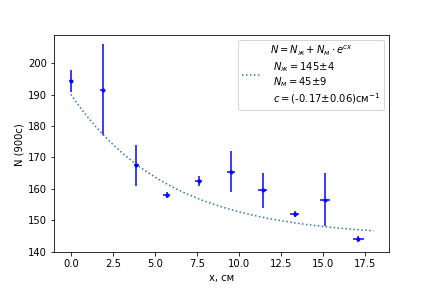
\includegraphics[scale=0.7]{N(x).png}}
\caption{Зависимость числа частиц, прошедших через слой свинца от толщины слоя}
\end{figure}
Измеренные значения в целом неплохо описываются зависимостью рассматриваемого вида (видим убывание числа прошедших через слой частиц с увеличением толщины слоя, скорость этого убывания уменьшается с увеличением толщины). Однако можно наблюдать некоторый разброс точек относительно тренда. Это связано с тем, что измерения носят статистический характер (зависят от того, сколько частиц излучения попало на прибор за заданное время). Поэтому для более точных результатов стоило провести больше измерений N для каждой заданной толщины (или увеличить время измерения). 
\item Найдем отношение интенсивнстей мягкой и жесткой компонент вторичного космического излучения
\begin{equation*}
    \frac{I_\text{м}}{I_\text{ж}} = \frac{\frac{N_\text{м}}{St}}{\frac{N_\text{ж}}{St}} = \frac{N_\text{м}}{N_\text{ж}},
    \sigma ({ \frac{I_\text{м}}{I_\text{ж}}}) =  \frac{I_\text{м}}{I_\text{ж}} \sqrt{{\frac{\sigma N_\text{м}}{N_\text{м}}}^2 + {\frac{\sigma N_\text{ж}}{N_\text{ж}}}^2}
\end{equation*}
\begin{equation*}
    \boxed{ \frac{I_\text{м}}{I_\text{ж}} = (0.32 \pm 0.06)}
\end{equation*}
\item
Сравним полученные значения с теоретическими данными. На уровне моря интенсивности мягкой и жесткой компонент $I_{\text{ж}} = 1.7 \cdot 10^{-2} \text{част} \cdot \text{см}^2 \cdot{c}^{-1}$ и $I_{\text{м}} = 0.7 \cdot 10^{-2} \text{част} \cdot \text{см}^2 \cdot{c}^{-1}$. Поэтому $\frac{I_{\text{м}}}{I_{\text{ж}}} \approx 0.4$\\
Экспериментальное значение согласуется с теоретическим (интенсивность жесткой компоненты выше). Небольшое численное отклонение могло возникнуть из-за того, что измерения проводились в лаборатории, поэтому часть мягкой компоненты излучения могла поглотиться зданием института. 
\end{itemize}

\section{Выводы}
\begin{itemize}
\item Вид зависимости интенсивности вторичного космического излучения от толщины поглощающего слоя свинца согласуется с теоретическим. 
\item Экспериментально установленное значение отношения интенсивностей мягкой и жесткой компонент вторичного космического излучения
\begin{equation*}
     \frac{I_\text{м}}{I_\text{ж}} = (0.32 \pm 0.06)
\end{equation*}
Большая погрешность $\approx 20\%$ результата связана с недостаточным количеством данных/с недостаточным временем проведения эксперимента.
\item Полученное значение немного меньше теоретического. Это связано с поглощением мягкой компоненты вторичного космического излучения зданием, в котором находится установка.
\end{itemize}
\end{document}